\documentclass[a4paper,12pt]{report}
\usepackage{amssymb}

\usepackage{ucs}
\usepackage[utf8x]{inputenc} % Input encoding for Greek characters
\usepackage[greek,english]{babel} % Language support

\newcommand{\en}{\selectlanguage{english}}
\newcommand{\gr}{\selectlanguage{greek}}

% \usepackage{algorithm2e}
% \usepackage{algorithm}
% \usepackage{algorithmic}
\usepackage{enumitem}
\usepackage{tcolorbox}
\tcbuselibrary{listingsutf8}
\usepackage{float}
\usepackage{amsmath}
\usepackage{graphicx} % For including images
\usepackage{titlesec} % Custom title formatting
\usepackage{fancyhdr} % For custom headers and footers
\usepackage{geometry} % For adjusting page margins

% Adjust the page margins to make content wider
\geometry{top=2.5cm, bottom=2.5cm, left=2.5cm, right=2.5cm}

% Redefine chapter formatting to make it smaller
\titleformat{\chapter}[display]
    {\normalfont\LARGE\bfseries} % Smaller size and bold for chapter heading
    {\chaptername\ \thechapter} % Chapter number format
    {15pt} % Space between chapter number and title
    {\bfseries} % Smaller size and bold for chapter title
\begin{document}

\begin{titlepage}
    \centering
    \vspace*{-3cm}
    % University logo
    \includegraphics[width=1\textwidth]{auth_logo.png} % Replace with your actual logo file

    % University name in Greek
    \textbf{\gr ΑΡΙΣΤΟΤΕΛΕΙΟ ΠΑΝΕΠΙΣΤΗΜΙΟ ΘΕΣΣΑΛΟΝΙΚΗΣ}
    \vspace{2cm}

    % Document title and subtitle in Greek
    \LARGE\textbf{\gr Ψηφιακή Επεξεργασία Εικόνας Αναφορά} \\
    \Large\normalfont{\gr Εργασία 1} \\
    \vspace{4cm}

    \gr
    \large
    \textbf{Διακολουκάς Δημήτριος} \\
    \textbf{AEM 10642}
    \vspace{2.5cm}

    \en
    \textit{Email: ddiakolou@ece.auth.gr}
\end{titlepage}

\gr
\tableofcontents

\chapter{Εισαγωγή και παρουσίαση εργασίας}

Η παρούσα εργασία ασχολείται με τεχνικές \textbf{εξισορρόπησης} και \textbf{αντιστοίχισης ιστογράμματος} \en (histogram equalization \& histogram matching) \gr σε γκρι εικόνες, με στόχο τη βελτίωση της αντίθεσης ή την προσαρμογή τους σε συγκεκριμένες κατανομές φωτεινότητας.

\vspace{0.3cm}

\hspace{-0.6cm}Αξιοποιούνται διαφορετικές εκδοχές των βασικών τεχνικών:

\begin{itemize}
    \item \en \textbf{Histogram Equalization}\gr, η οποία αποσκοπεί στην ισοκατανομή της φωτεινότητας των pixels σε μία εικόνα, οδηγώντας σε καλύτερη εκμετάλλευση της δυναμικής περιοχής \en (dynamic range)\gr.
    
    \item \en \textbf{Histogram Matching}\gr, κατά την οποία μια εικόνα τροποποιείται ώστε η κατανομή της φωτεινότητάς της να πλησιάζει αυτήν μιας εικόνας αναφοράς.

    \item Και οι δύο τεχνικές υλοποιούνται με διαφορετικές μεθοδολογίες: \en \textit{greedy}\gr, \en \textit{non-greedy}\gr, και \en \textit{post-disturbance}\gr, καθεμία από τις οποίες επιχειρεί διαφορετικό βαθμό προσέγγισης στην επιθυμητή κατανομή.
\end{itemize}

\hspace{-0.6cm}Η εργασία αυτή στο μάθημα \textbf{Ψηφιακή Επεξεργασία Εικόνας} ακολουθεί πλήρως τις προδιαγραφές που δίνονται στην εκφώνηση. Η υλοποίηση έγινε εξολοκλήρου σε γλώσσα \en Python \gr με την χρήση πακέτων όπως \en Numpy, Matplotlib \gr και \en PIL\gr. 

\vspace{0.3cm}

\hspace{-0.6cm}Τα επιμέρους τμήματα της εργασίας περιλαμβάνουν:

\begin{enumerate}
    \item Υλοποίηση βασικών συναρτήσεων ιστογράμματος στο αρχείο \en \texttt{hist\_utils.py}\gr.
    \item Υλοποίηση αλγορίθμων εξισορρόπησης και αντιστοίχισης ιστογράμματος στο \en \texttt{hist\_modif.py}\gr.
    \item Πρόγραμμα επίδειξης των μεθόδων και παραγωγής γραφημάτων στο \en \texttt{demo.py}\gr.
    \item Αναλυτική αναφορά, με εξηγήσεις των συναρτήσεων, εικόνες, ιστογράμματα και σχόλια στα αποτελέσματα.
\end{enumerate}

\hspace{-0.6cm}Στην εργασία αξιολογούνται συγκριτικά οι τρεις προσσεγγίσεις εξισορρόπησης και αντιστοίχισης ιστογράμματος ως προς την κατανομή εξόδου, την οπτική ποιότητα και την ακρίβεια ως προς τον στόχο. Τα αποτελέσματα παρουσιάζονται γραφικά μέσω αυτόματης παραγωγής διαγραμμάτων, με χρήση των εικόνων \en \texttt{input\_img.jpg} \gr και \en \texttt{ref\_img.png} \gr που δόθηκαν ως \en input \gr δεδομένα στον κώδικα.

\chapter{Μέθοδοι Εξισορρόπησης Ιστογράμματος}

Η εξισορρόπηση ιστογράμματος \en (\textit{histogram equalization}) \gr αποτελεί μια βασική τεχνική βελτίωσης της αντίθεσης εικόνας. Στόχος της είναι η ανακατανομή των τιμών φωτεινότητας έτσι ώστε η έξοδος να κατανέμεται όσο το δυνατόν πιο ομοιόμορφα στο εύρος τιμών.

\section{Μαθηματικό Υπόβαθρο}

Για μια εικόνα $f(n_1, n_2)$ με $L$ διακριτές στάθμες $f_0, f_1, \dots, f_{L-1}$, ορίζουμε την πιθανότητα εμφάνισης της $f_i$ ως:
\en 
\[
p_f(f_i) = \frac{\text{count}(f_i)}{N}
\]
\gr

\hspace{-0.6cm}Η εξισορρόπηση ιστογράμματος στοχεύει στη δημιουργία εικόνας $g(n_1, n_2)$ με νέα κατανομή $p_g$ τέτοια ώστε:

\[
p_g(g_j) \approx \frac{1}{L_g}, \quad \forall j
\]

\hspace{-0.6cm}όπου $g_j$ οι στάθμες εξόδου και $L_g$ ο αριθμός τους.

\hspace{-0.6cm}Εναλλακτικά, για συνεχές μοντέλο, αν θεωρήσουμε bins $b_i = [f_i, f_{i+1})$, τότε:
\en
\[
p_f(b_i) = \frac{\text{pixels in } b_i}{N}
\]
\gr
και στόχος είναι κάθε \en bin\gr εξόδου να έχει περίπου ίσο πλήθος \en pixels\gr.



\section{\en Greedy Histogram Equalization\gr}

Η μέθοδος αυτή είναι άπληστη και αντιστοιχίζει τις $f_i$ σε $g_j$ μέχρι να καλυφθεί το \en \texttt{desired[j]}\gr, έπειτα προχωρά στην επόμενη στάθμη.

\begin{tcolorbox}[colback=gray!5!white, colframe=black!75!black, title=Ψευδοκώδικας \en Greedy Equalization\gr]
\en 
\begin{verbatim}
j = 0
filled = 0
For every (f_i, count_i):
    mapping[f_i] = g_j
    filled += count_i
    If filled >= desired[j] and j < len(g) - 1:
        j += 1
        filled = 0
\end{verbatim}
\end{tcolorbox}
\gr

\begin{tcolorbox}[colback=gray!5!white, colframe=black!75!black, title=Παρατήρηση]
Απλή υλοποίηση, αλλά μπορεί να οδηγήσει σε απότομες αλλαγές στην έξοδο, ειδικά αν υπάρχουν ανισοκατανεμημένες στάθμες εισόδου.
\end{tcolorbox}


\section{\en Non-Greedy Histogram Equalization\gr}

Εδώ εξετάζεται πότε πρέπει να αλλάξει η έξοδος ώστε να περιοριστεί η απόκλιση από το επιθυμητό πλήθος:
\en
\[
\text{deficiency}_j = \texttt{desired}[j] - \sum_{i} \texttt{count}(f_i)
\]
\gr
Το μέγεθος \en \texttt{desired[j]} \gr αντιστοιχεί στο επιθυμητό πλήθος δειγμάτων που θα πρέπει να χαρτογραφηθούν στη στάθμη εξόδου $g_j$. Στην περίπτωση εξισορρόπησης ως προς ομοιόμορφη κατανομή, αυτό ισούται ιδανικά με:
\en
\[
\texttt{desired}[j] = \left\lfloor \frac{N}{L_g} \right\rfloor
\]
\gr

\hspace{-0.6cm}όπου $N$ είναι ο συνολικός αριθμός δειγμάτων \en (pixels) \gr της εικόνας και $L_g$ το πλήθος των στάθμεων εξόδου.

\begin{tcolorbox}[colback=gray!5!white, colframe=black!75!black, title=Ψευδοκώδικας \en Non-Greedy Equalization\gr]
\en
\begin{verbatim}
For every g_j:
    taken = 0
    If f_i available:
        mapping[f_i] = g_j
        taken += count_i
    While deficiency >= count_i / 2:
        mapping[f_i] = g_j
        taken += count_i
        i += 1
\end{verbatim}
\end{tcolorbox}
\gr
\begin{tcolorbox}[colback=gray!5!white, colframe=black!40!black, title=Πλεονέκτημα]
Παρέχει πιο «λεία» κατανομή και μειώνει τη συγκέντρωση πολλών εισόδων στην ίδια έξοδο.
\end{tcolorbox}


\section{\en Post-Disturbance Equalization}
\gr
Σε αυτή τη μέθοδο προστίθεται λίγος τυχαίος «θόρυβος» στις τιμές των \en pixels \gr ώστε να μην υπάρχουν πολλές ίδιες τιμές. Αυτό βοηθά στο να κατανέμονται τα \en pixels \gr πιο σωστά στις στάθμες εξόδου:

\[
\hat{f}(n_1, n_2) = f(n_1, n_2) + \nu(n_1, n_2), \quad \nu \sim \mathcal{U}(-d/2, d/2)
\]

\begin{tcolorbox}[colback=gray!5!white, colframe=black!75!black, title=Ψευδοκώδικας \en Post-Disturbance Equalization\gr]
\en
\begin{verbatim}
flat = img.ravel()
disturbed = flat + uniform(-d/2, d/2)
indices = argsort(disturbed)

For every j:
    out[indices[start:end]] = g[j]
\end{verbatim}
\end{tcolorbox}
\gr

\begin{tcolorbox}[colback=gray!5!white, colframe=black!75!black, title=Ιδιαιτερότητα]
Καταργεί την ανάγκη ρητής αντιστοίχισης $f_i \mapsto g_j$ και οδηγεί σε πολύ καλή προσέγγιση της κατανομής εξόδου.
\end{tcolorbox}

\chapter{Ανάλυση Υλοποιημένων Συναρτήσεων}

Σε αυτό το κεφάλαιο περιγράφονται αναλυτικά οι βασικές συναρτήσεις που υλοποιήθηκαν στα αρχεία \en \texttt{hist\_utils.py} \gr και \en \texttt{hist\_modif.py}\gr. Οι συναρτήσεις αυτές αποτελούν τον βασικό πυρήνα για τον υπολογισμό και την τροποποίηση ιστογραμμάτων εικόνας, τόσο για εξισορρόπηση όσο και για αντιστοίχιση για κάθε μία από τις μεθόδους που αναλύσαμε σε προηγούμενο κεφάλαιο.

\section{Υπολογισμός Ιστογράμματος \en (\texttt{calculate\_hist\_of\_img})\gr}

Η συνάρτηση αυτή δέχεται ως είσοδο μια \en 2D \gr εικόνα επιπέδων του γκρι και επιστρέφει το ιστόγραμμά της, είτε σε απόλυτες τιμές \en (\texttt{counts}) \gr είτε κανονικοποιημένο \en (\texttt{relative frequencies})\gr, με βάση την τιμή της παραμέτρου \en \texttt{return\_normalized}\gr.

\begin{itemize}
  \item \textbf{Είσοδος:} Εικόνα $f$ διαστάσεων $H \times W$, με τιμές σε $[0,1]$
  \item \textbf{Έξοδος:} \en dictionary \gr $h$ με κλειδιά τις διακριτές τιμές $f_i$ και τιμές είτε τις σχετικές συχνότητες είτε το πλήθος εμφάνισης.
\end{itemize}

\begin{tcolorbox}[colback=gray!5!white, colframe=black!75!black, title=Ψευδοκώδικας \en \texttt{calculate\_hist\_of\_img}\gr]
\en 
\begin{verbatim}
flatten = img.ravel()
values, counts = unique(flatten, return_counts=True)
if return_normalized:
    counts = counts / total_pixels
return dict(zip(values, counts))
\end{verbatim}
\end{tcolorbox}
\gr

\hspace{-0.6cm}Η λειτουργία της συνάρτησης είναι θεμελιώδης για όλες τις επόμενες μετατροπές και η υλοποίηση της βρίσκεται στο αρχείο \en hist\_utils.py\gr.

\section{Εφαρμογή Μετασχηματισμού Εντάσεων \newline \en (\texttt{apply\_hist\_modification\_transform})\gr}

Η συνάρτηση εφαρμόζει έναν έτοιμο μετασχηματισμό $f_i \rightarrow g_j$ σε κάθε \en pixel \gr της εικόνας.

\begin{itemize}
  \item \textbf{Είσοδος:} Εικόνα $f$ και μετασχηματισμός \en \texttt{modification\_transform}\gr, δηλαδή \en dictionary \gr που αντιστοιχεί στάθμες $f_i$ σε τιμές εξόδου $g_j$.
  \item \textbf{Έξοδος:} Νέα εικόνα $g(n_1, n_2)$ με τιμές $g_j$.
\end{itemize}

\hspace{-0.6cm}Η συνάρτηση ταξινομεί τα κλειδιά του λεξικού και χρησιμοποιεί \en \texttt{searchsorted} \gr για γρήγορη ανάθεση τιμών.

\begin{tcolorbox}[colback=gray!5!white, colframe=black!75!black, title=Ψευδοκώδικας \en \texttt{apply\_hist\_modification\_transform}\gr]
\en 
\begin{verbatim}
flatten = img.ravel()
sort keys and values of transform
indices = searchsorted(sorted_keys, flatten)
output = sorted_vals[indices]
reshape to original image shape
\end{verbatim}
\end{tcolorbox}
\gr

\hspace{-0.6cm}Αν η είσοδος περιλαμβάνει στάθμες που δεν καλύπτονται από τον μετασχηματισμό, αποτυγχάνει με \en \texttt{KeyError}\gr. H υλοποίηση της βρίσκεται στο αρχείο \en hist\_utils.py\gr.

\section{Μετατροπή Επιθυμητής Κατανομής σε Απόλυτα \en Counts (\texttt{\_desired\_counts})\gr}

Η συνάρτηση \en \texttt{\_desired\_counts} \gr λαμβάνει ως είσοδο ένα \en dictionary \gr κατανομής πιθανοτήτων (π.χ. ομοιόμορφη ή προερχόμενη από άλλη εικόνα) και μετατρέπει τις σχετικές συχνότητες σε απόλυτους αριθμούς pixels.

\begin{itemize}
  \item \textbf{Είσοδος:} $p_{\text{\en ref\gr}}(g_j)$ (σχετική κατανομή), πλήθος $N$ όλων των \en pixels\gr.
  \item \textbf{Έξοδος:} Ταξινομημένες στάθμες $g_j$ και επιθυμητά πλήθη $c_j \in \mathbb{N}$ τέτοια ώστε $\sum_j c_j = N$.
\end{itemize}

\hspace{-0.6cm}Η στρογγυλοποίηση προς τα κάτω μπορεί να αφήσει υπόλοιπο. Αυτό κατανέμεται στα bins με το μεγαλύτερο δεκαδικό μέρος.

\begin{tcolorbox}[colback=gray!5!white, colframe=black!75!black, title=Ψευδοκώδικας \en \texttt{\_desired\_counts}\gr]
\en
\begin{verbatim}
ideal = p * total_pixels
counts = floor(ideal)
residual = total_pixels - sum(counts)
distribute +1 to bins with largest fractional remainders
return sorted(g), corresponding c
\end{verbatim}
\end{tcolorbox}
\gr

\hspace{-0.6cm}Η υλοποίηση της βοηθητικής συνάρτησης αυτής βρίσκεται στο αρχείο \en hist\_modif.py\gr.

\section{Κύριες Συναρτήσεις Υψηλού Επιπέδου}

\subsection*{Υλοποίηση \en \texttt{perform\_hist\_modification}\gr}

Η συνάρτηση αυτή είναι ο βασικός ενδιάμεσος μηχανισμός. Με βάση τη μέθοδο \en (\texttt{mode}) \gr και το επιθυμητό ιστόγραμμα, αποφασίζει ποια προσέγγιση τροποποίησης θα εφαρμοστεί \en (greedy, non-greedy \gr ή \en post-disturbance\gr). Χρησιμοποιεί:

\begin{itemize}
  \item \en \texttt{\_desired\_counts} \gr για παραγωγή $g_j$ και $c_j$
  \item \en \texttt{calculate\_hist\_of\_img} \gr για εξαγωγή του πραγματικού ιστογράμματος
  \item \en \texttt{apply\_hist\_modification\_transform} \gr για τελική ανάθεση
\end{itemize}

\subsection*{Υλοποίηση \en \texttt{perform\_hist\_eq}\gr}

Εκτελεί εξισορρόπηση ιστογράμματος ως προς ομοιόμορφη κατανομή.
 
\[
p_{\text{\en ref\gr}}(g_j) = \frac{1}{L_g}, \quad \text{για κάθε } j = 0, \dots, L_g - 1
\]

\hspace{-0.6cm}Παράγει $L_g$ ισαπέχουσες στάθμες και αναθέτει $N/L_g$ \en pixels \gr σε κάθε μία μέσω της \newline \en \texttt{perform\_hist\_modification}\gr.

\subsection*{Υλοποίηση \en \texttt{perform\_hist\_matching}\gr}

Πραγματοποιεί αντιστοίχιση ιστογράμματος \en (histogram matching) \gr ως προς κατανομή αναφοράς από δεύτερη εικόνα. Εξάγει το κανονικοποιημένο ιστόγραμμα της εικόνας-αναφοράς και καλεί την ίδια \en \texttt{perform\_hist\_modification} \gr για να επιτευχθεί η αντιστοίχιση.

\begin{tcolorbox}[colback=gray!5!white, colframe=black!75!black, title=Δομή χρήσης \en \texttt{perform\_hist\_matching}\gr]
\en
\begin{verbatim}
ref_hist = calculate_hist_of_img(reference_image, True)
output = perform_hist_modification(input_image, ref_hist, mode)
\end{verbatim}
\end{tcolorbox}
\gr

\chapter{Εκτέλεση προγράμματος, αποτελέσματα, συμπεράσματα}

\section{Εκτέλεση του \en \texttt{demo.py}\gr}

Η υλοποίηση που παρουσιάστηκε συνοδεύεται από το αρχείο \en \texttt{demo.py}\gr, το οποίο αποτελεί το βασικό \en script \gr για την επίδειξη της λειτουργίας των συναρτήσεων εξισορρόπησης και αντιστοίχισης ιστογράμματος που αναπτύχθηκαν στα \en \texttt{hist\_utils.py} \gr και \en \texttt{hist\_modif.py}\gr.

Το πρόγραμμα διαβάζει δύο εικόνες:
\begin{itemize}
  \item \en \texttt{input\_img.jpg} \gr -- η αρχική εικόνα
  \item \en \texttt{ref\_img.jpg} \gr -- εικόνα αναφοράς για την αντιστοίχιση ιστογράμματος
\end{itemize}

\hspace{-0.6cm}Κάθε εικόνα φορτώνεται σε \en grayscale \gr μορφή με τιμές ανακλιμάκωσης στο διάστημα $[0,1]$ μέσω της βιβλιοθήκης \en PIL\gr. Για κάθε μια από τις τρεις μεθόδους \en (\texttt{greedy}, \texttt{non-greedy}, \texttt{post-disturbance}) \gr εφαρμόζεται:
\begin{enumerate}
  \item εξισορρόπηση ιστογράμματος με αναφορά ομοιόμορφη κατανομή,
  \item αντιστοίχιση ιστογράμματος προς το ιστόγραμμα της εικόνας αναφοράς.
\end{enumerate}

\hspace{-0.6cm}Για κάθε έξοδο παράγεται εικόνα και το αντίστοιχο γράφημα ιστογράμματος.

\section{Παραγόμενα Αποτελέσματα}

Το πρόγραμμα αποθηκεύει αυτόματα τα αποτελέσματα στον ίδιο φάκελο με τα αρχεία κώδικα. Για κάθε μέθοδο δημιουργούνται:
\begin{itemize}
  \item \textbf{Εικόνες εξόδου:} συγκρίσεις της αρχικής εικόνας με την εξισωμένη ή αντιστοιχισμένη.
  \item \textbf{Ιστόγραμμα:} σχετική συχνότητα τιμών πριν και μετά την επεξεργασία.
\end{itemize}

\hspace{-0.6cm}Παρακάτω παρατίθενται παραδείγματα αποτελεσμάτων \textbf{εξισορρόπησης ιστογράμματος} με τις τρεις τεχνικές και έγινε \en testing \gr για τιμές \en \(L_g\) = [15, 256, 1200] \gr καθώς και αποτελέσματα αντιστοίχισης μετέπειτα:

\begin{figure}[H]
\centering
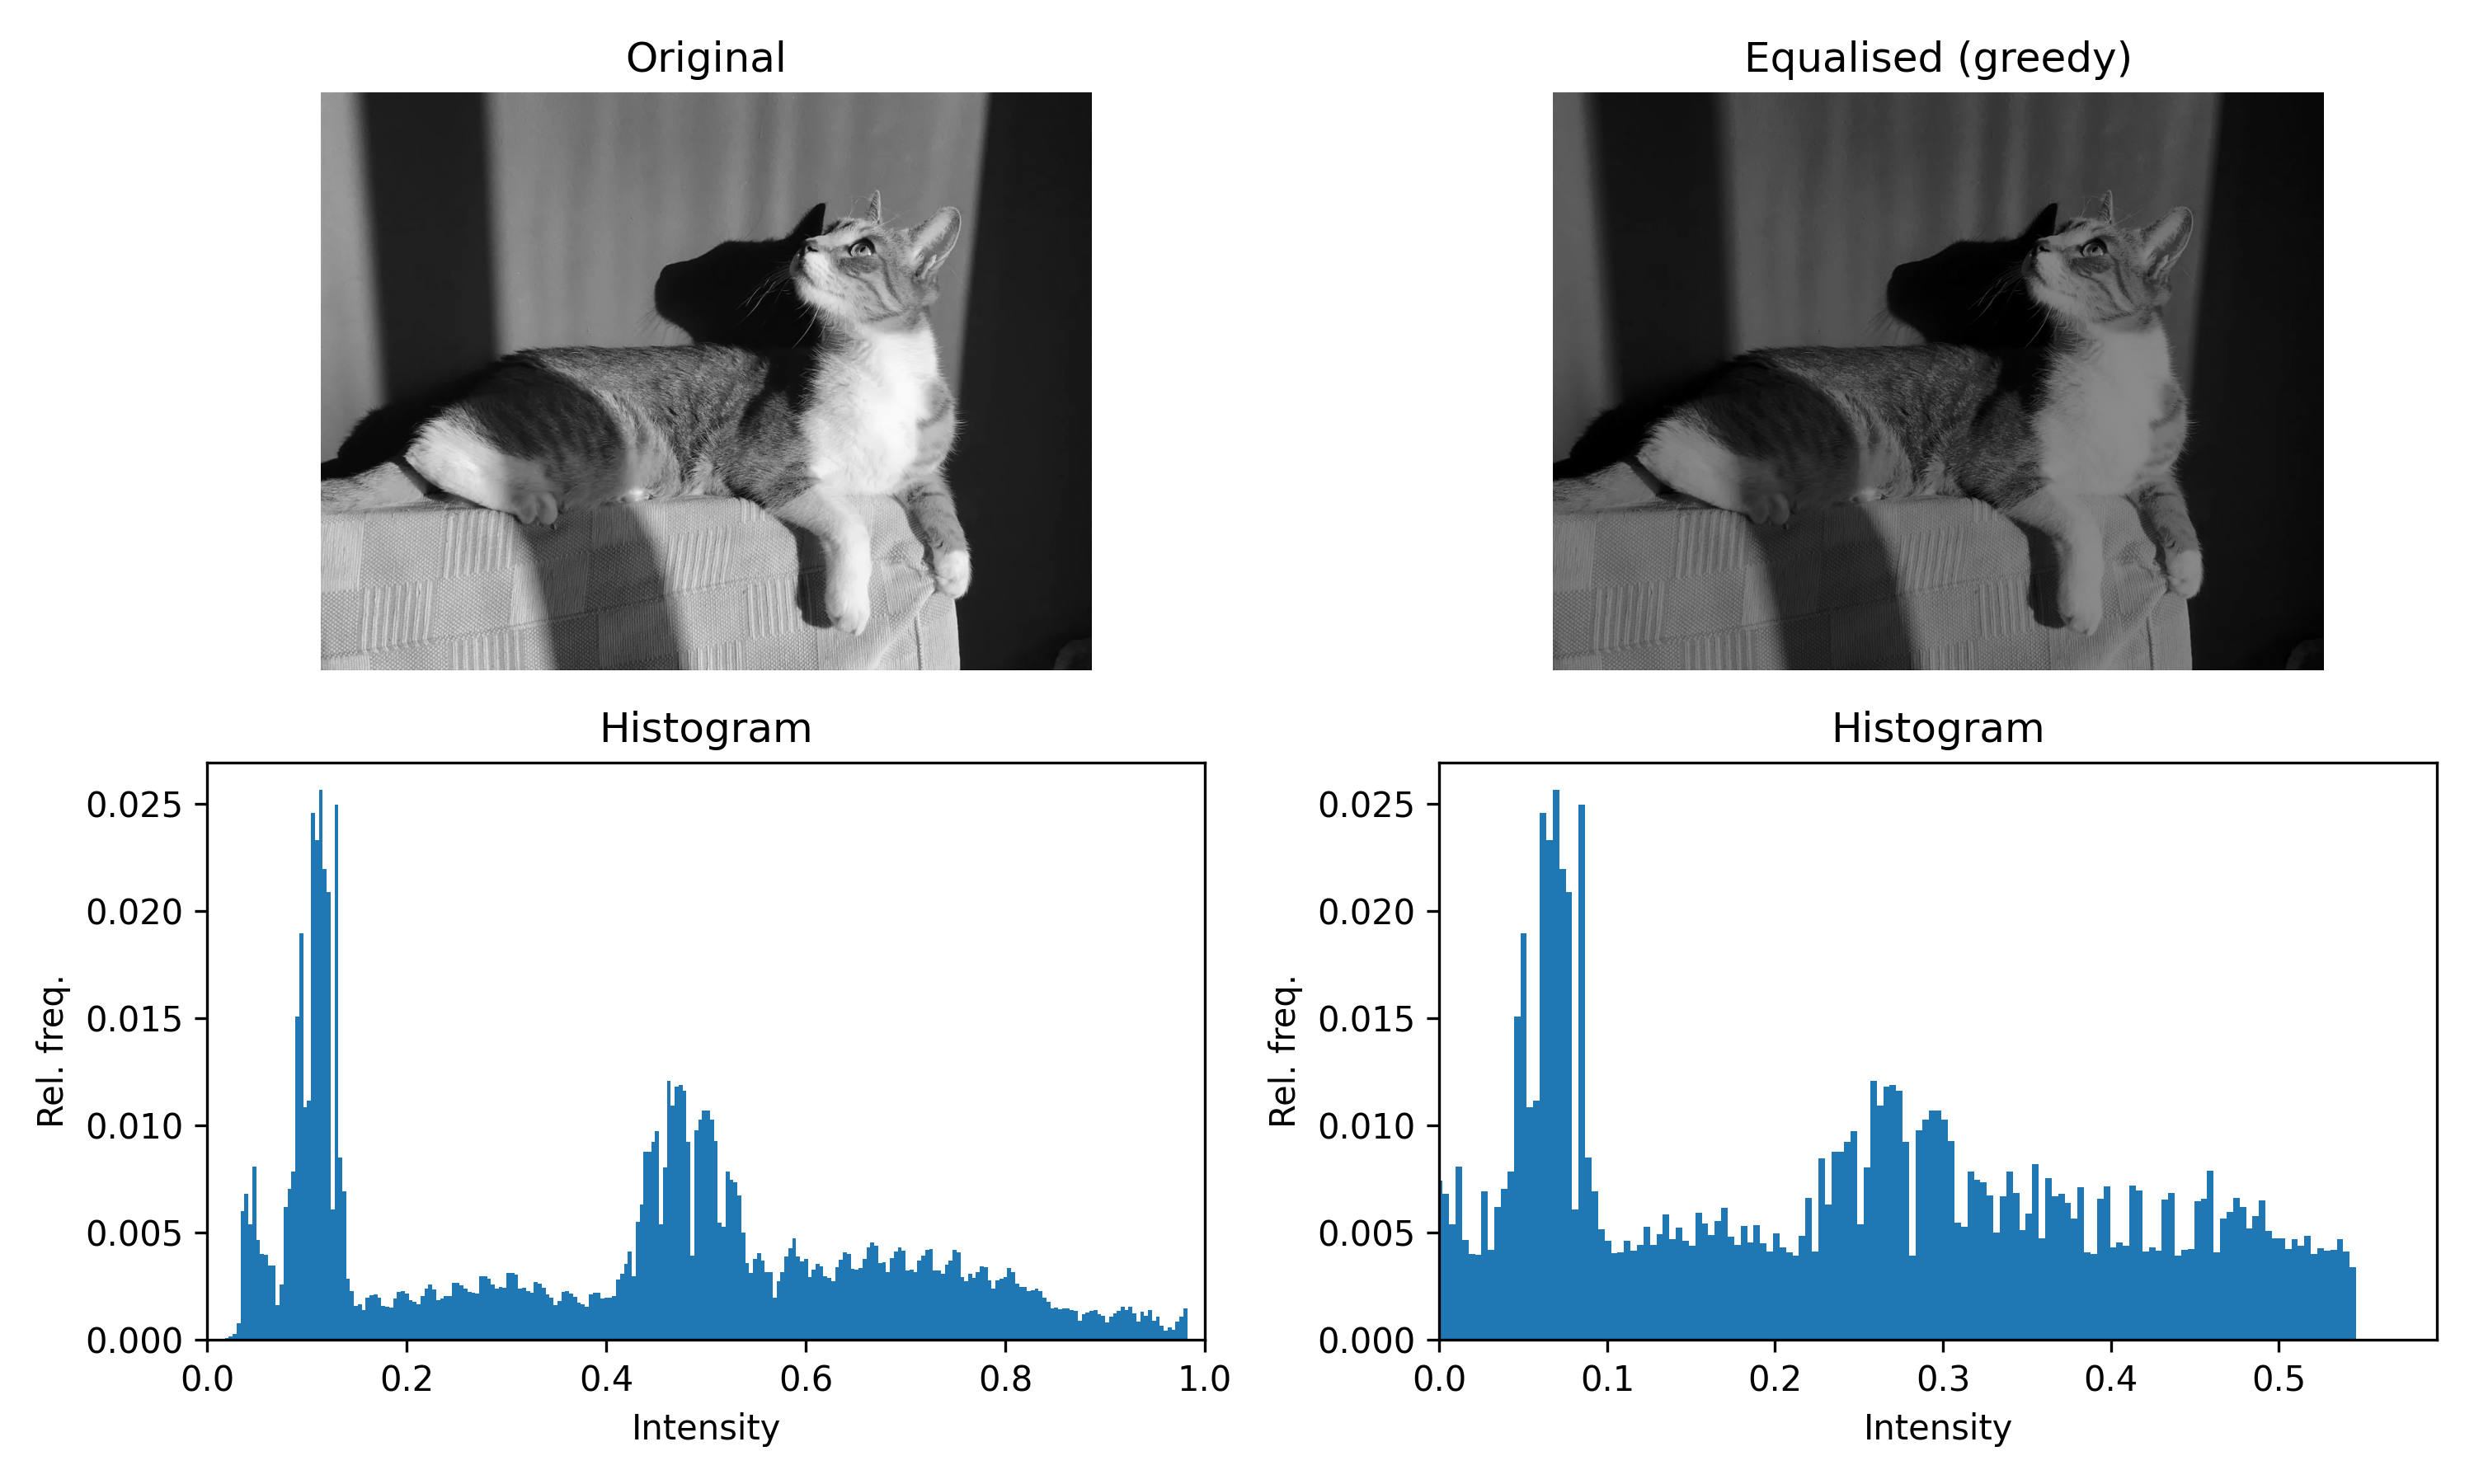
\includegraphics[width=0.9\textwidth]{eq_greedy.png}
\caption{Εξισορρόπηση με τη μέθοδο \en Greedy\gr. Η έξοδος προσεγγίζει μια ισοκατανομή (\en \(L_g\) = 256\gr).}
\end{figure}

\begin{figure}[H]
\centering
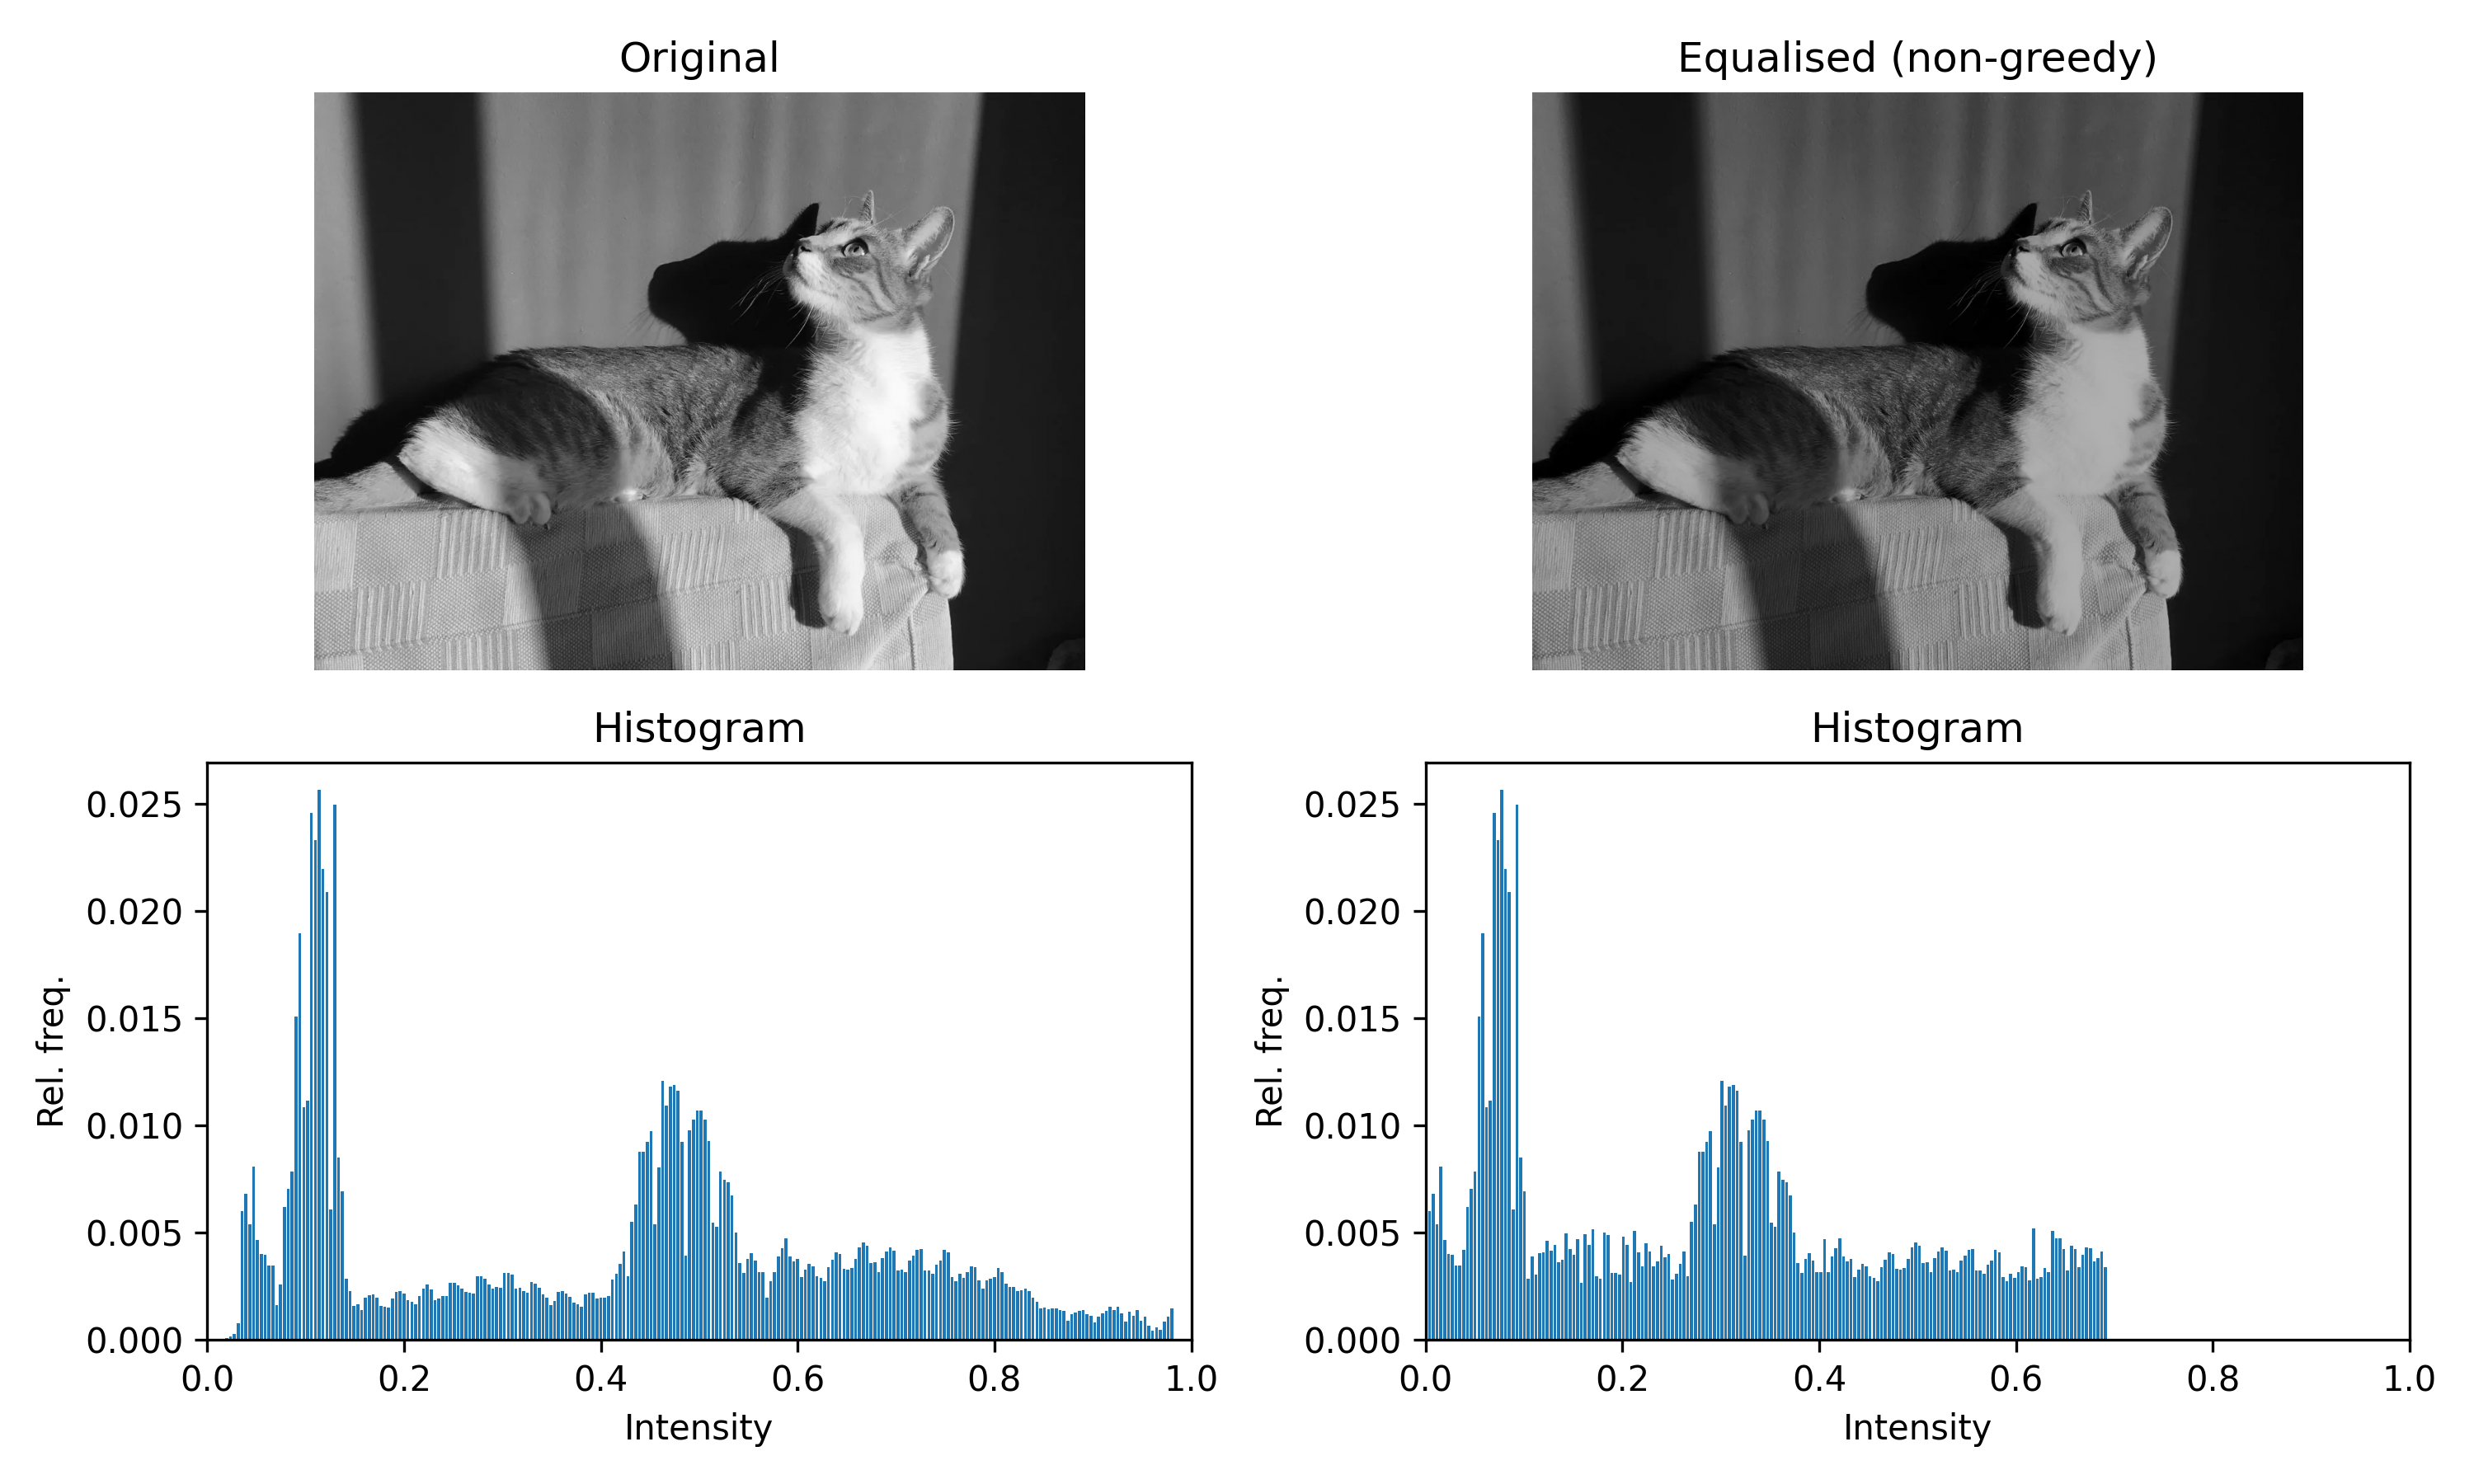
\includegraphics[width=0.9\textwidth]{eq_non-greedy.png}
\caption{Εξισορρόπηση με τη μέθοδο \en Non-Greedy\gr. Μειώνεται η υπερ-εκχώρηση στάθμης (\en \(L_g\) = 256\gr).}
\end{figure}

\begin{figure}[H]
\centering
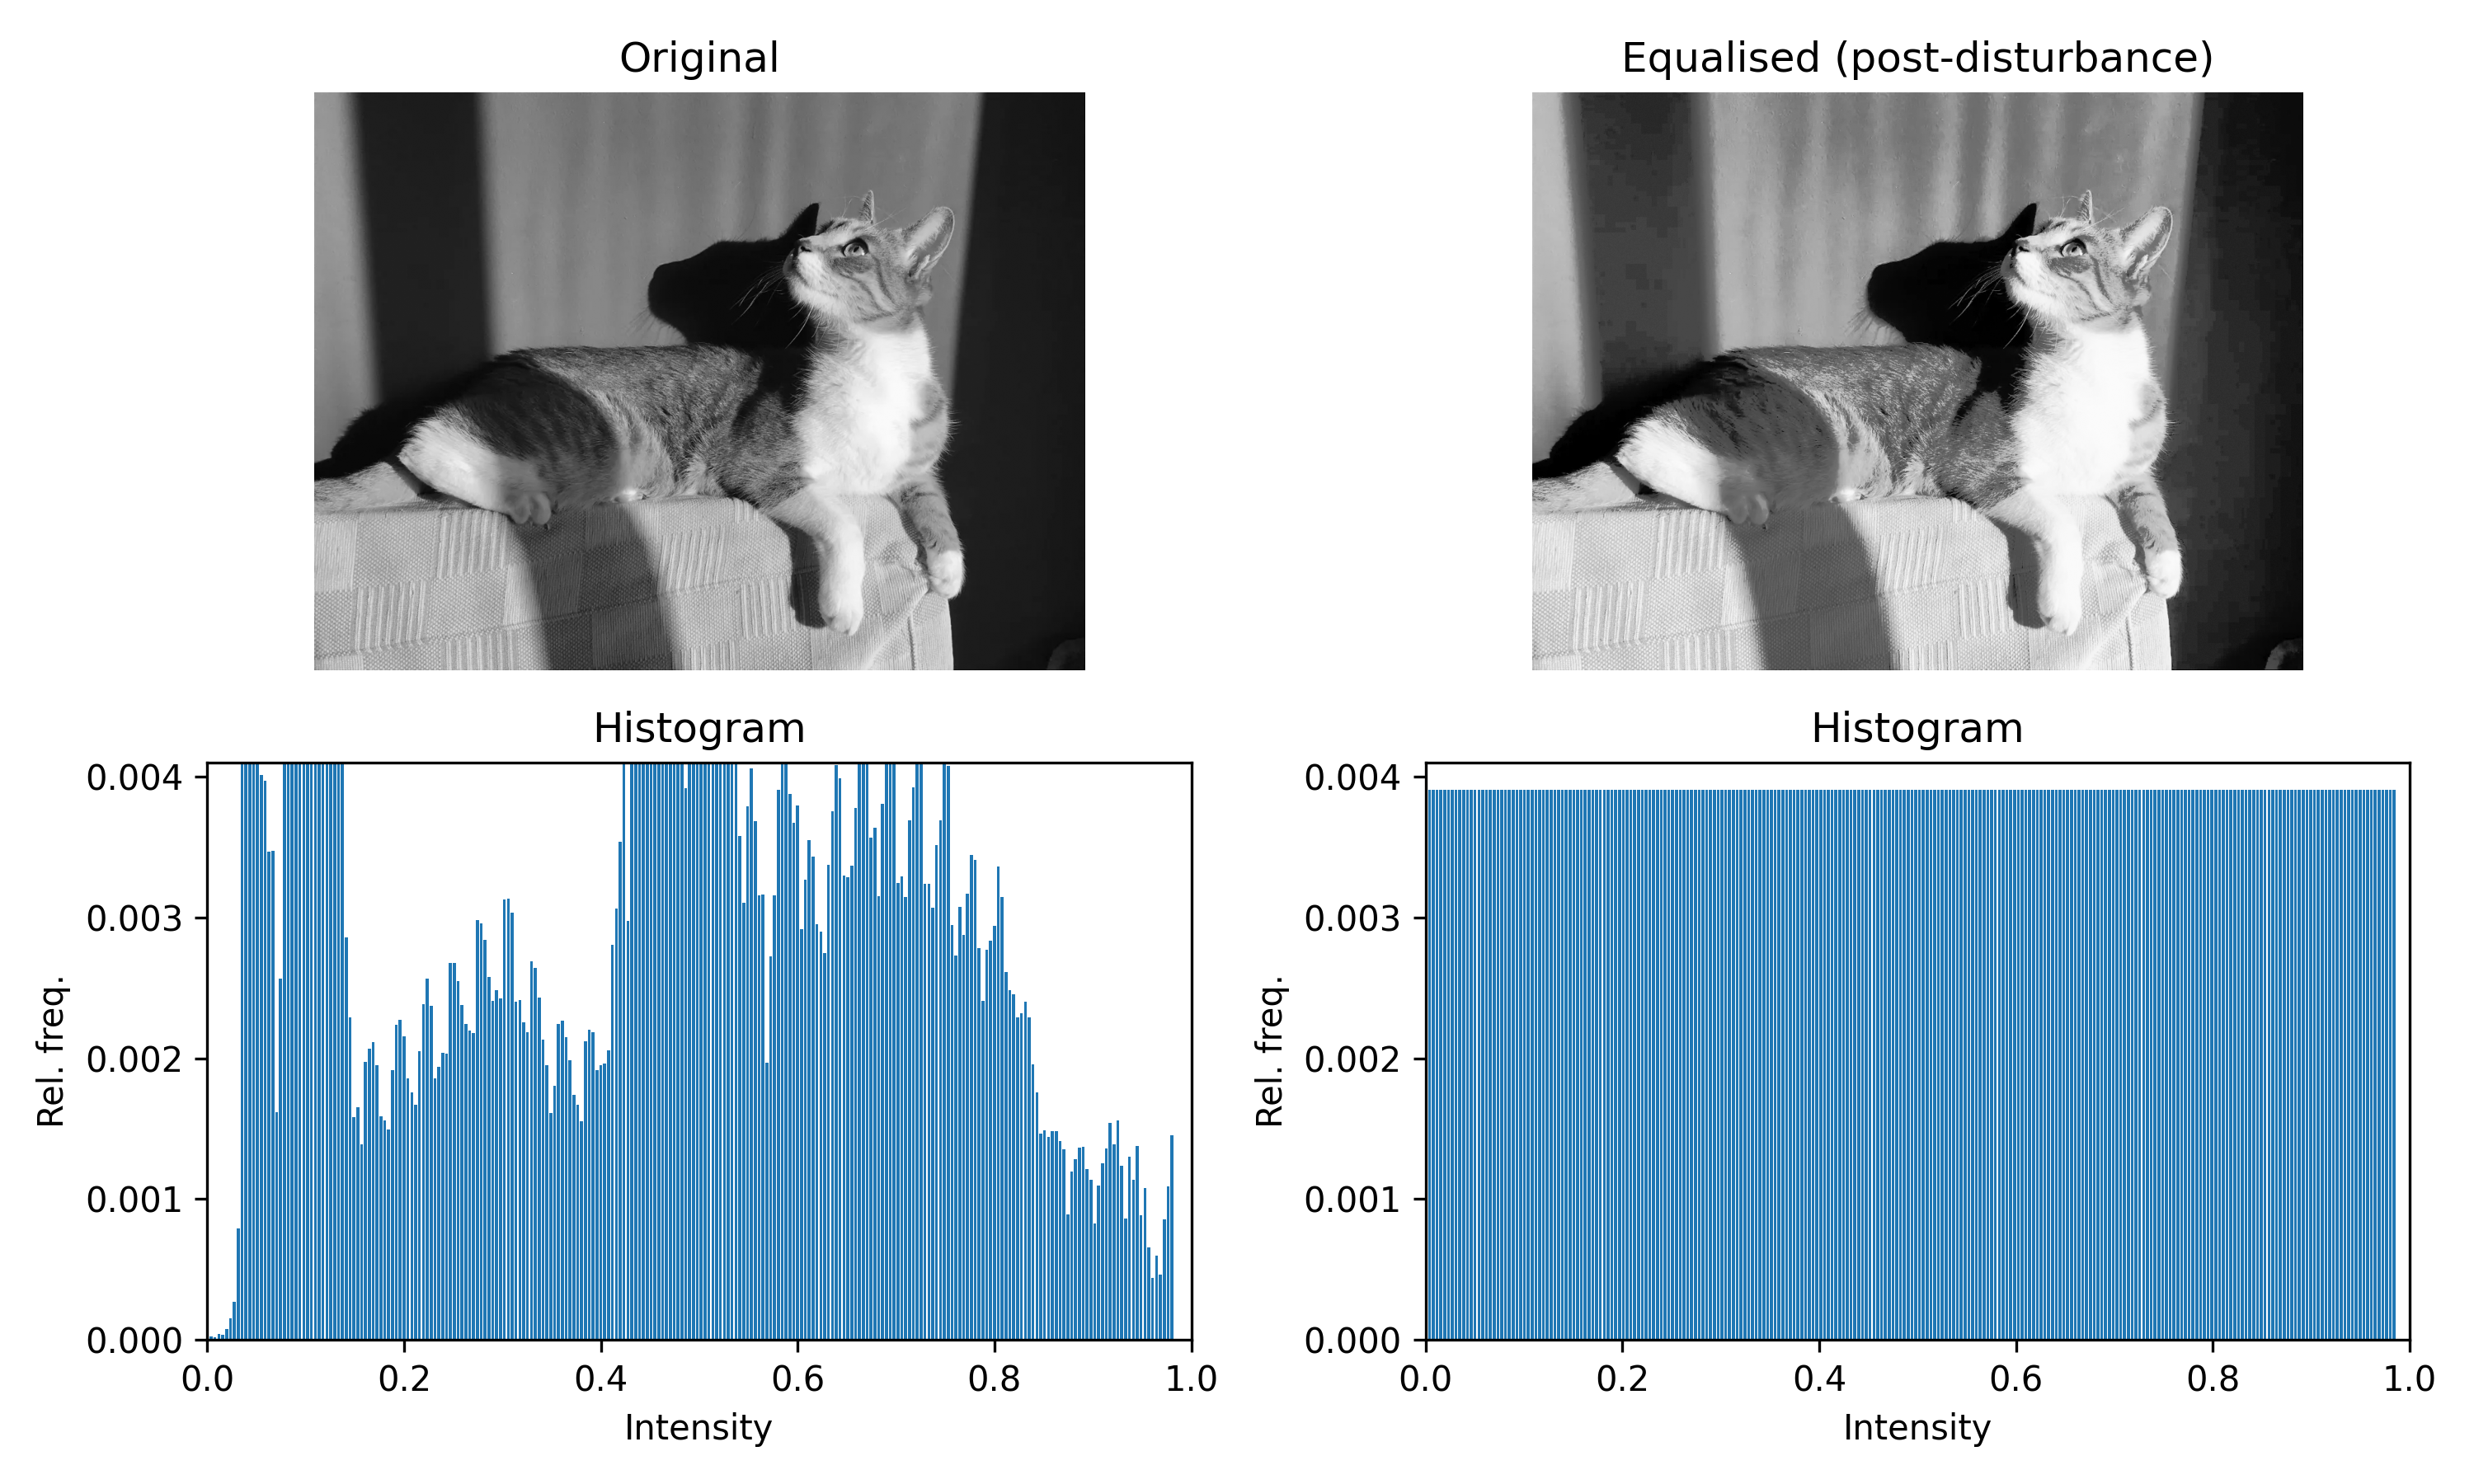
\includegraphics[width=0.9\textwidth]{eq_post-disturbance.png}
\caption{Εξισορρόπηση με την τεχνική \en Post-Disturbance\gr. Προκύπτει ισορροπημένο ιστόγραμμα (\en \(L_g\) = 256\gr).}
\end{figure}

\begin{figure}[H]
\centering
\includegraphics[width=0.9\textwidth]{eq_greedy0.png}
\caption{Εξισορρόπηση με τη μέθοδο \en Greedy\gr. Η έξοδος προσεγγίζει μια ισοκατανομή (\en \(L_g\) = 15\gr).}
\end{figure}

\begin{figure}[H]
\centering
\includegraphics[width=0.9\textwidth]{eq_non-greedy0.png}
\caption{Εξισορρόπηση με τη μέθοδο \en Non-Greedy\gr. Μειώνεται η υπερ-εκχώρηση στάθμης (\en \(L_g\) = 15\gr).}
\end{figure}

\begin{figure}[H]
\centering
\includegraphics[width=0.9\textwidth]{eq_post-disturbance0.png}
\caption{Εξισορρόπηση με την τεχνική \en Post-Disturbance\gr. Προκύπτει ισορροπημένο ιστόγραμμα (\en \(L_g\) = 15\gr).}
\end{figure}

\begin{figure}[H]
\centering
\includegraphics[width=0.9\textwidth]{eq_greedy2.png}
\caption{Εξισορρόπηση με τη μέθοδο \en Greedy\gr. Η έξοδος προσεγγίζει μια ισοκατανομή (\en \(L_g\) = 1200\gr).}
\end{figure}

\begin{figure}[H]
\centering
\includegraphics[width=0.9\textwidth]{eq_non-greedy2.png}
\caption{Εξισορρόπηση με τη μέθοδο \en Non-Greedy\gr. Μειώνεται η υπερ-εκχώρηση στάθμης (\en \(L_g\) = 1200\gr).}
\end{figure}

\begin{figure}[H]
\centering
\includegraphics[width=0.9\textwidth]{eq_post-disturbance2.png}
\caption{Εξισορρόπηση με την τεχνική \en Post-Disturbance\gr. Προκύπτει ισορροπημένο ιστόγραμμα (\en \(L_g\) = 1200\gr).}
\end{figure}

\vspace{0.5cm}

\hspace{-0.6cm}Ακολουθούν και τα αποτελέσματα από τη διαδικασία \textbf{αντιστοίχισης ιστογράμματος}:

\begin{figure}[H]
\centering
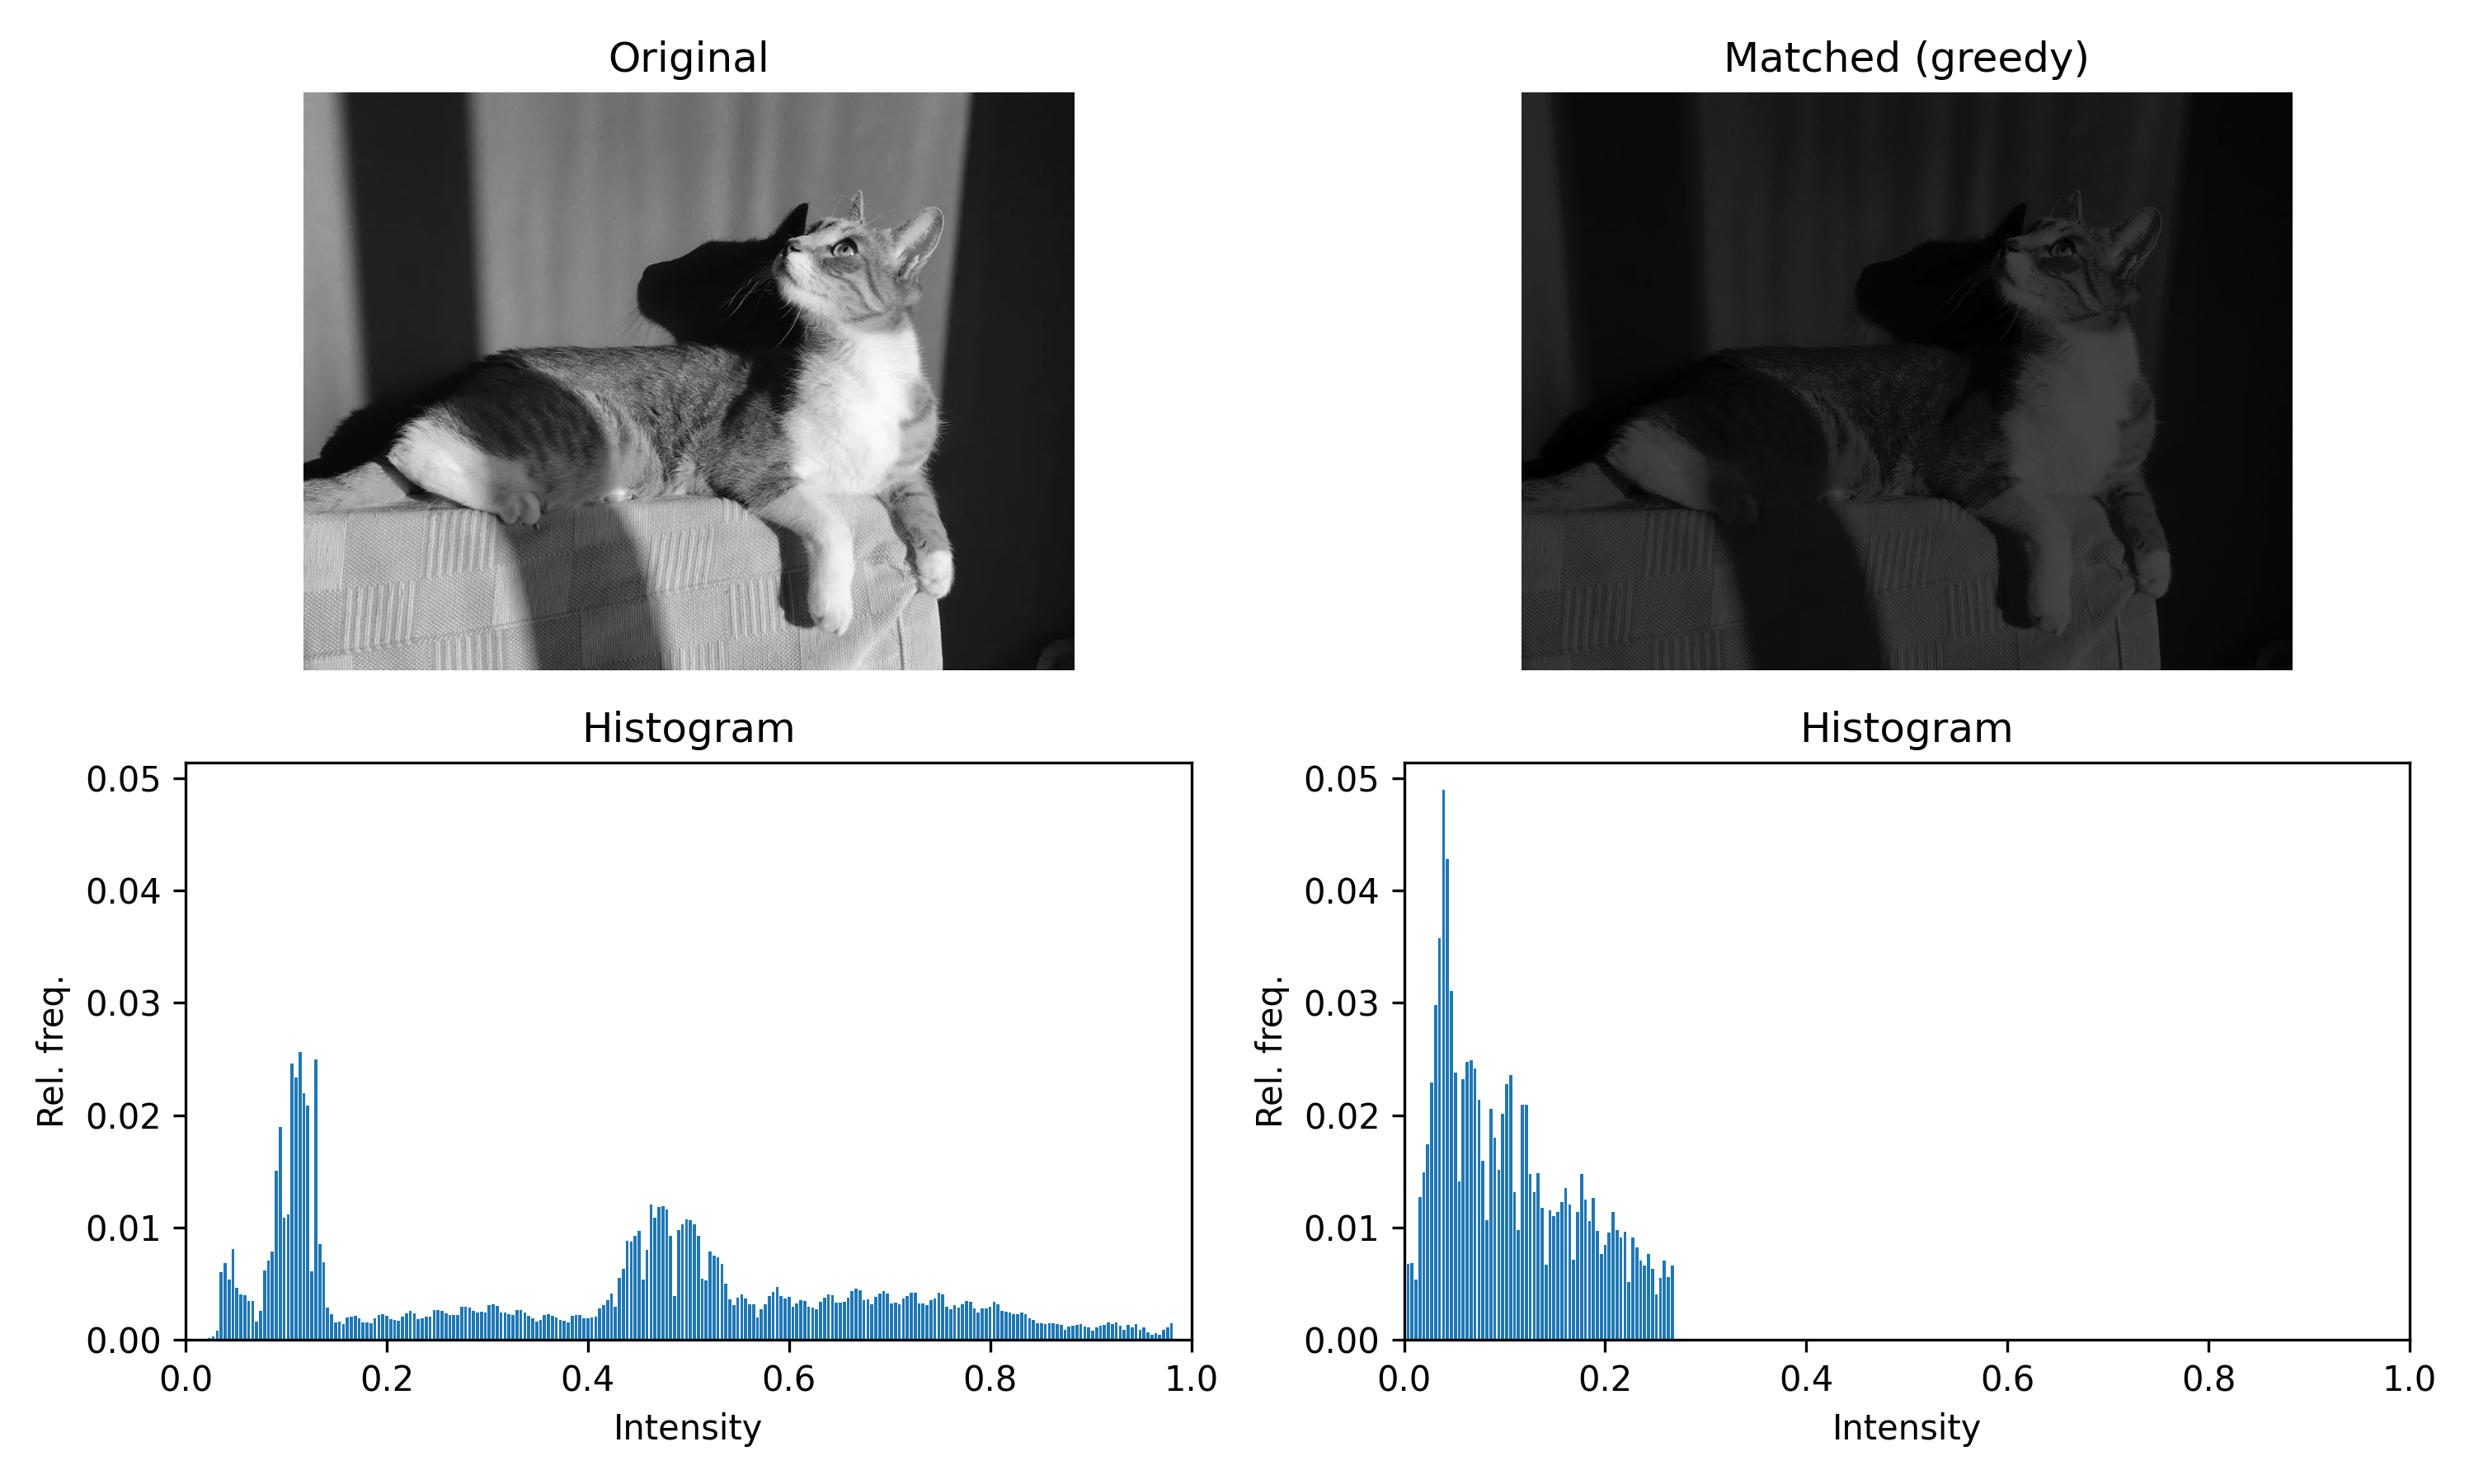
\includegraphics[width=0.9\textwidth]{match_greedy.png}
\caption{Αντιστοίχιση ιστογράμματος με χρήση της \en greedy \gr προσέγγισης.}
\end{figure}

\begin{figure}[H]
\centering
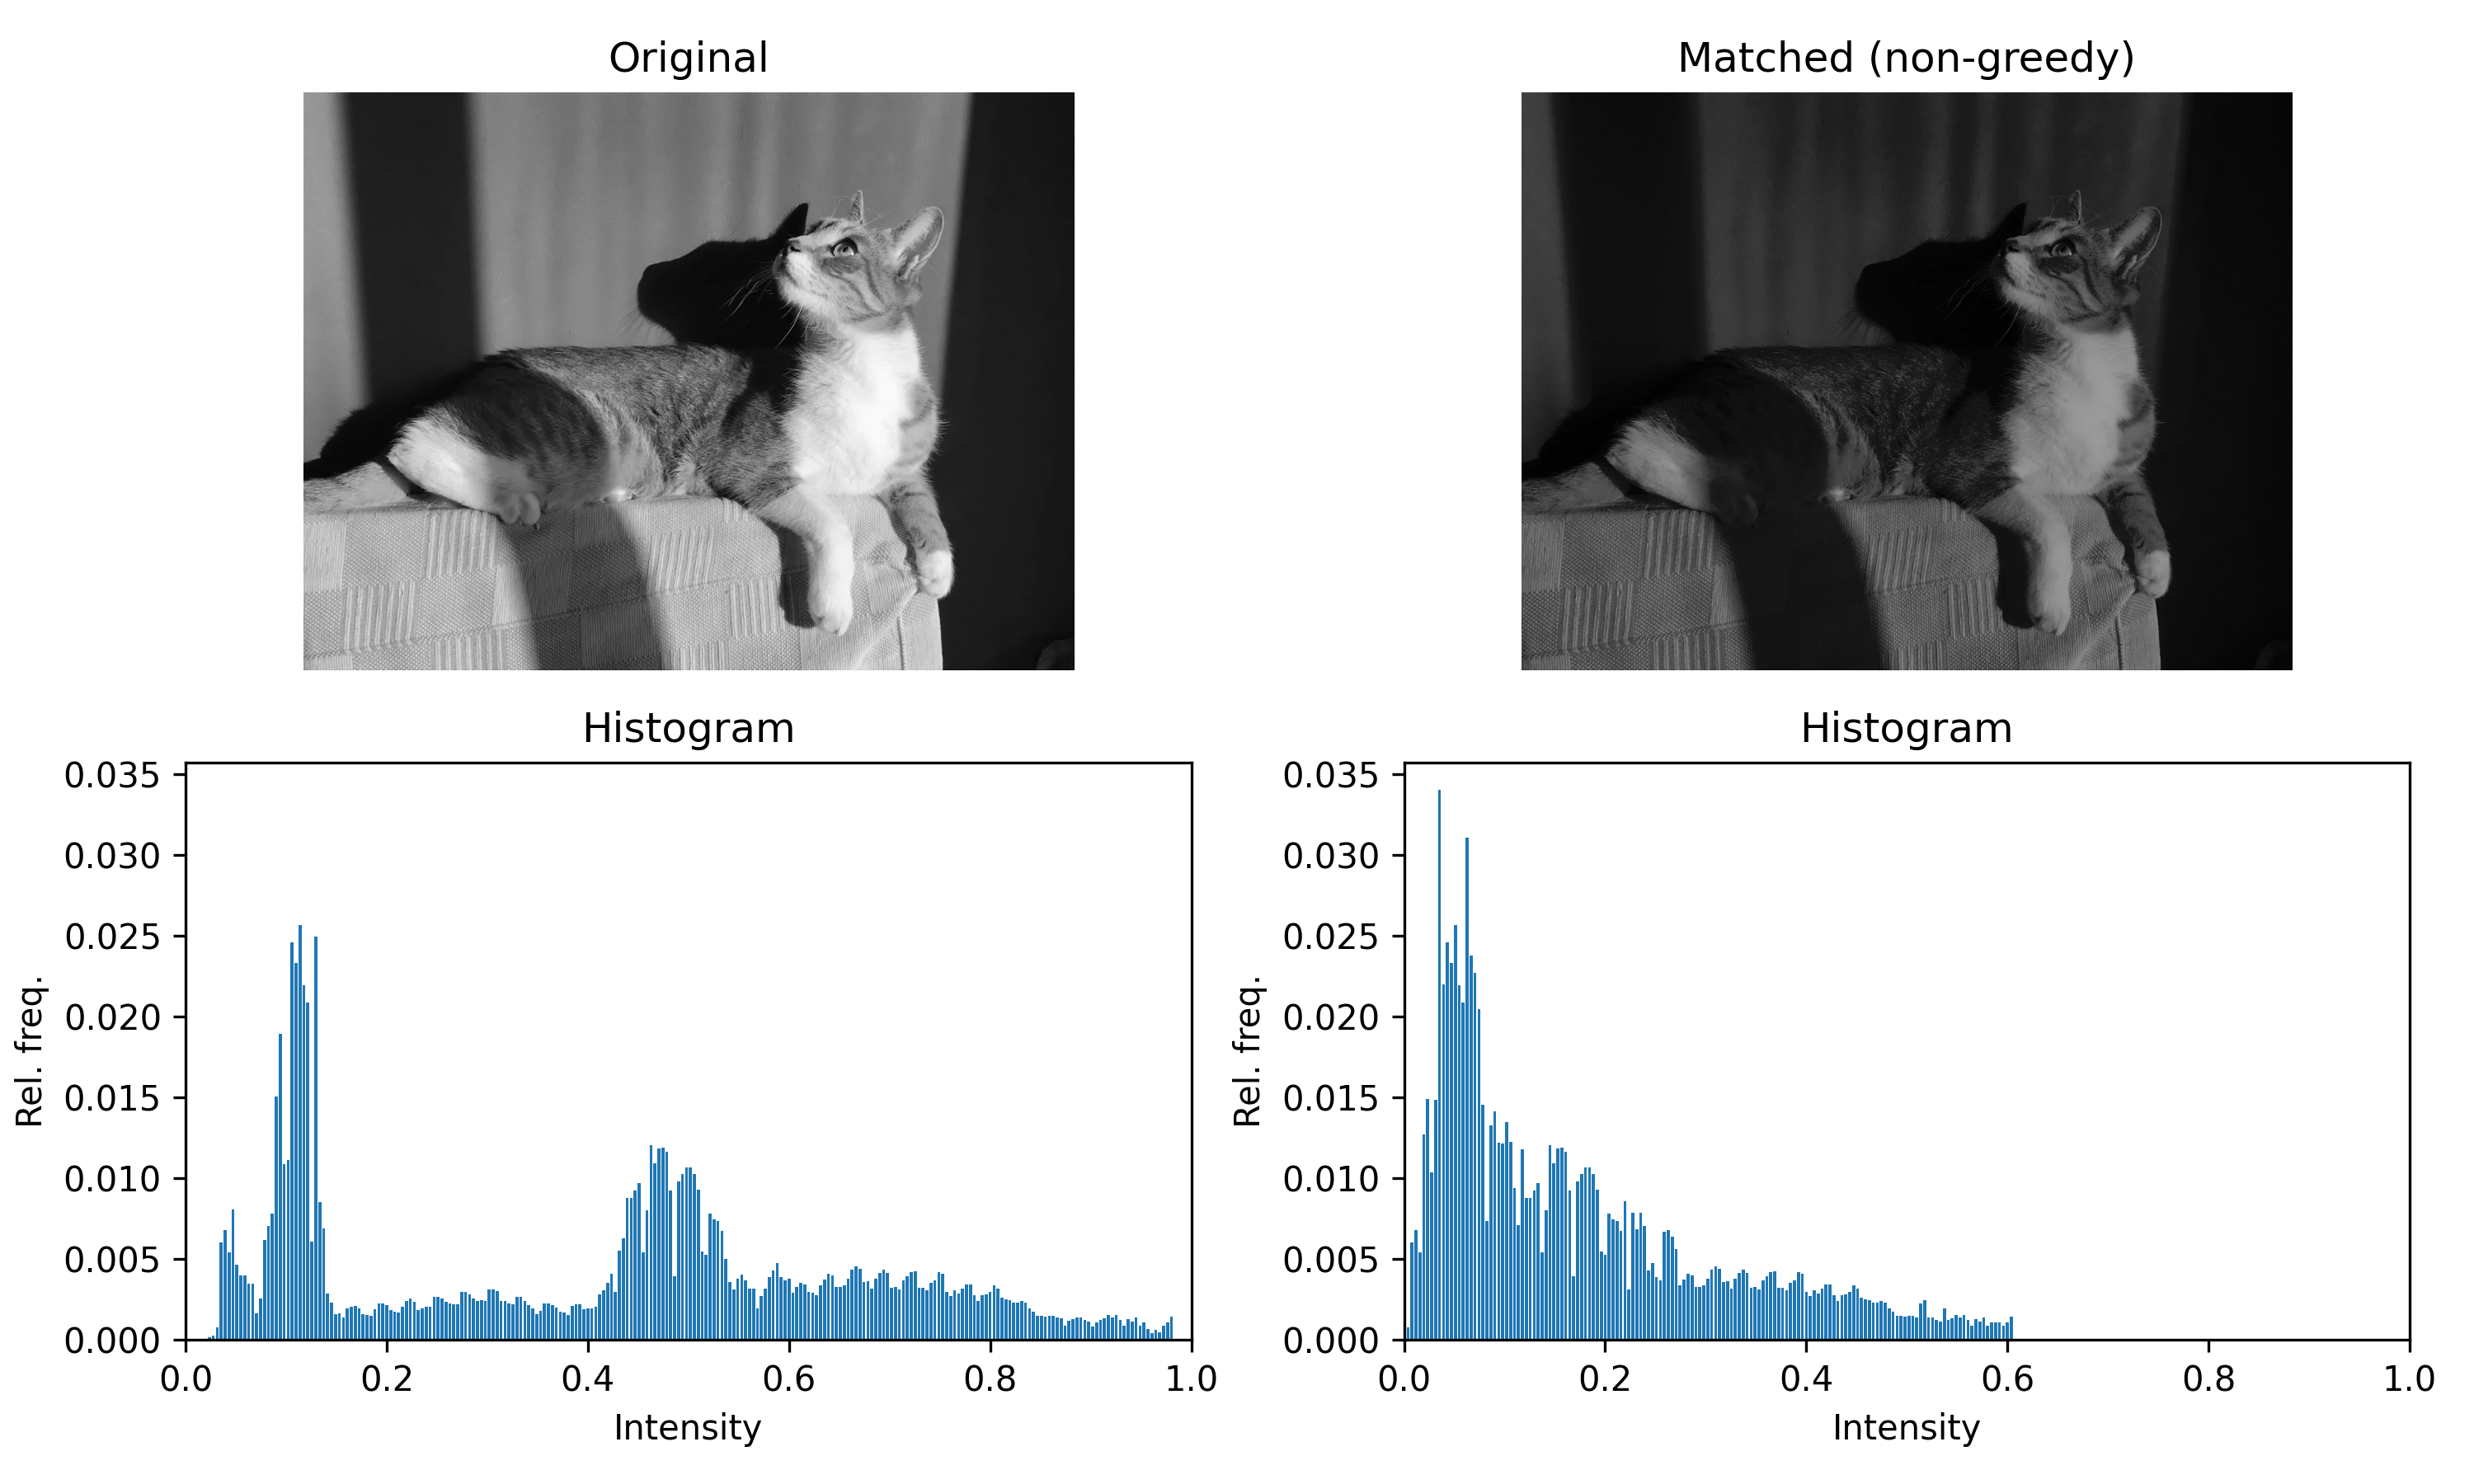
\includegraphics[width=0.9\textwidth]{match_non-greedy.png}
\caption{Αντιστοίχιση ιστογράμματος με \en non-greedy \gr προσέγγιση.}
\end{figure}

\begin{figure}[H]
\centering
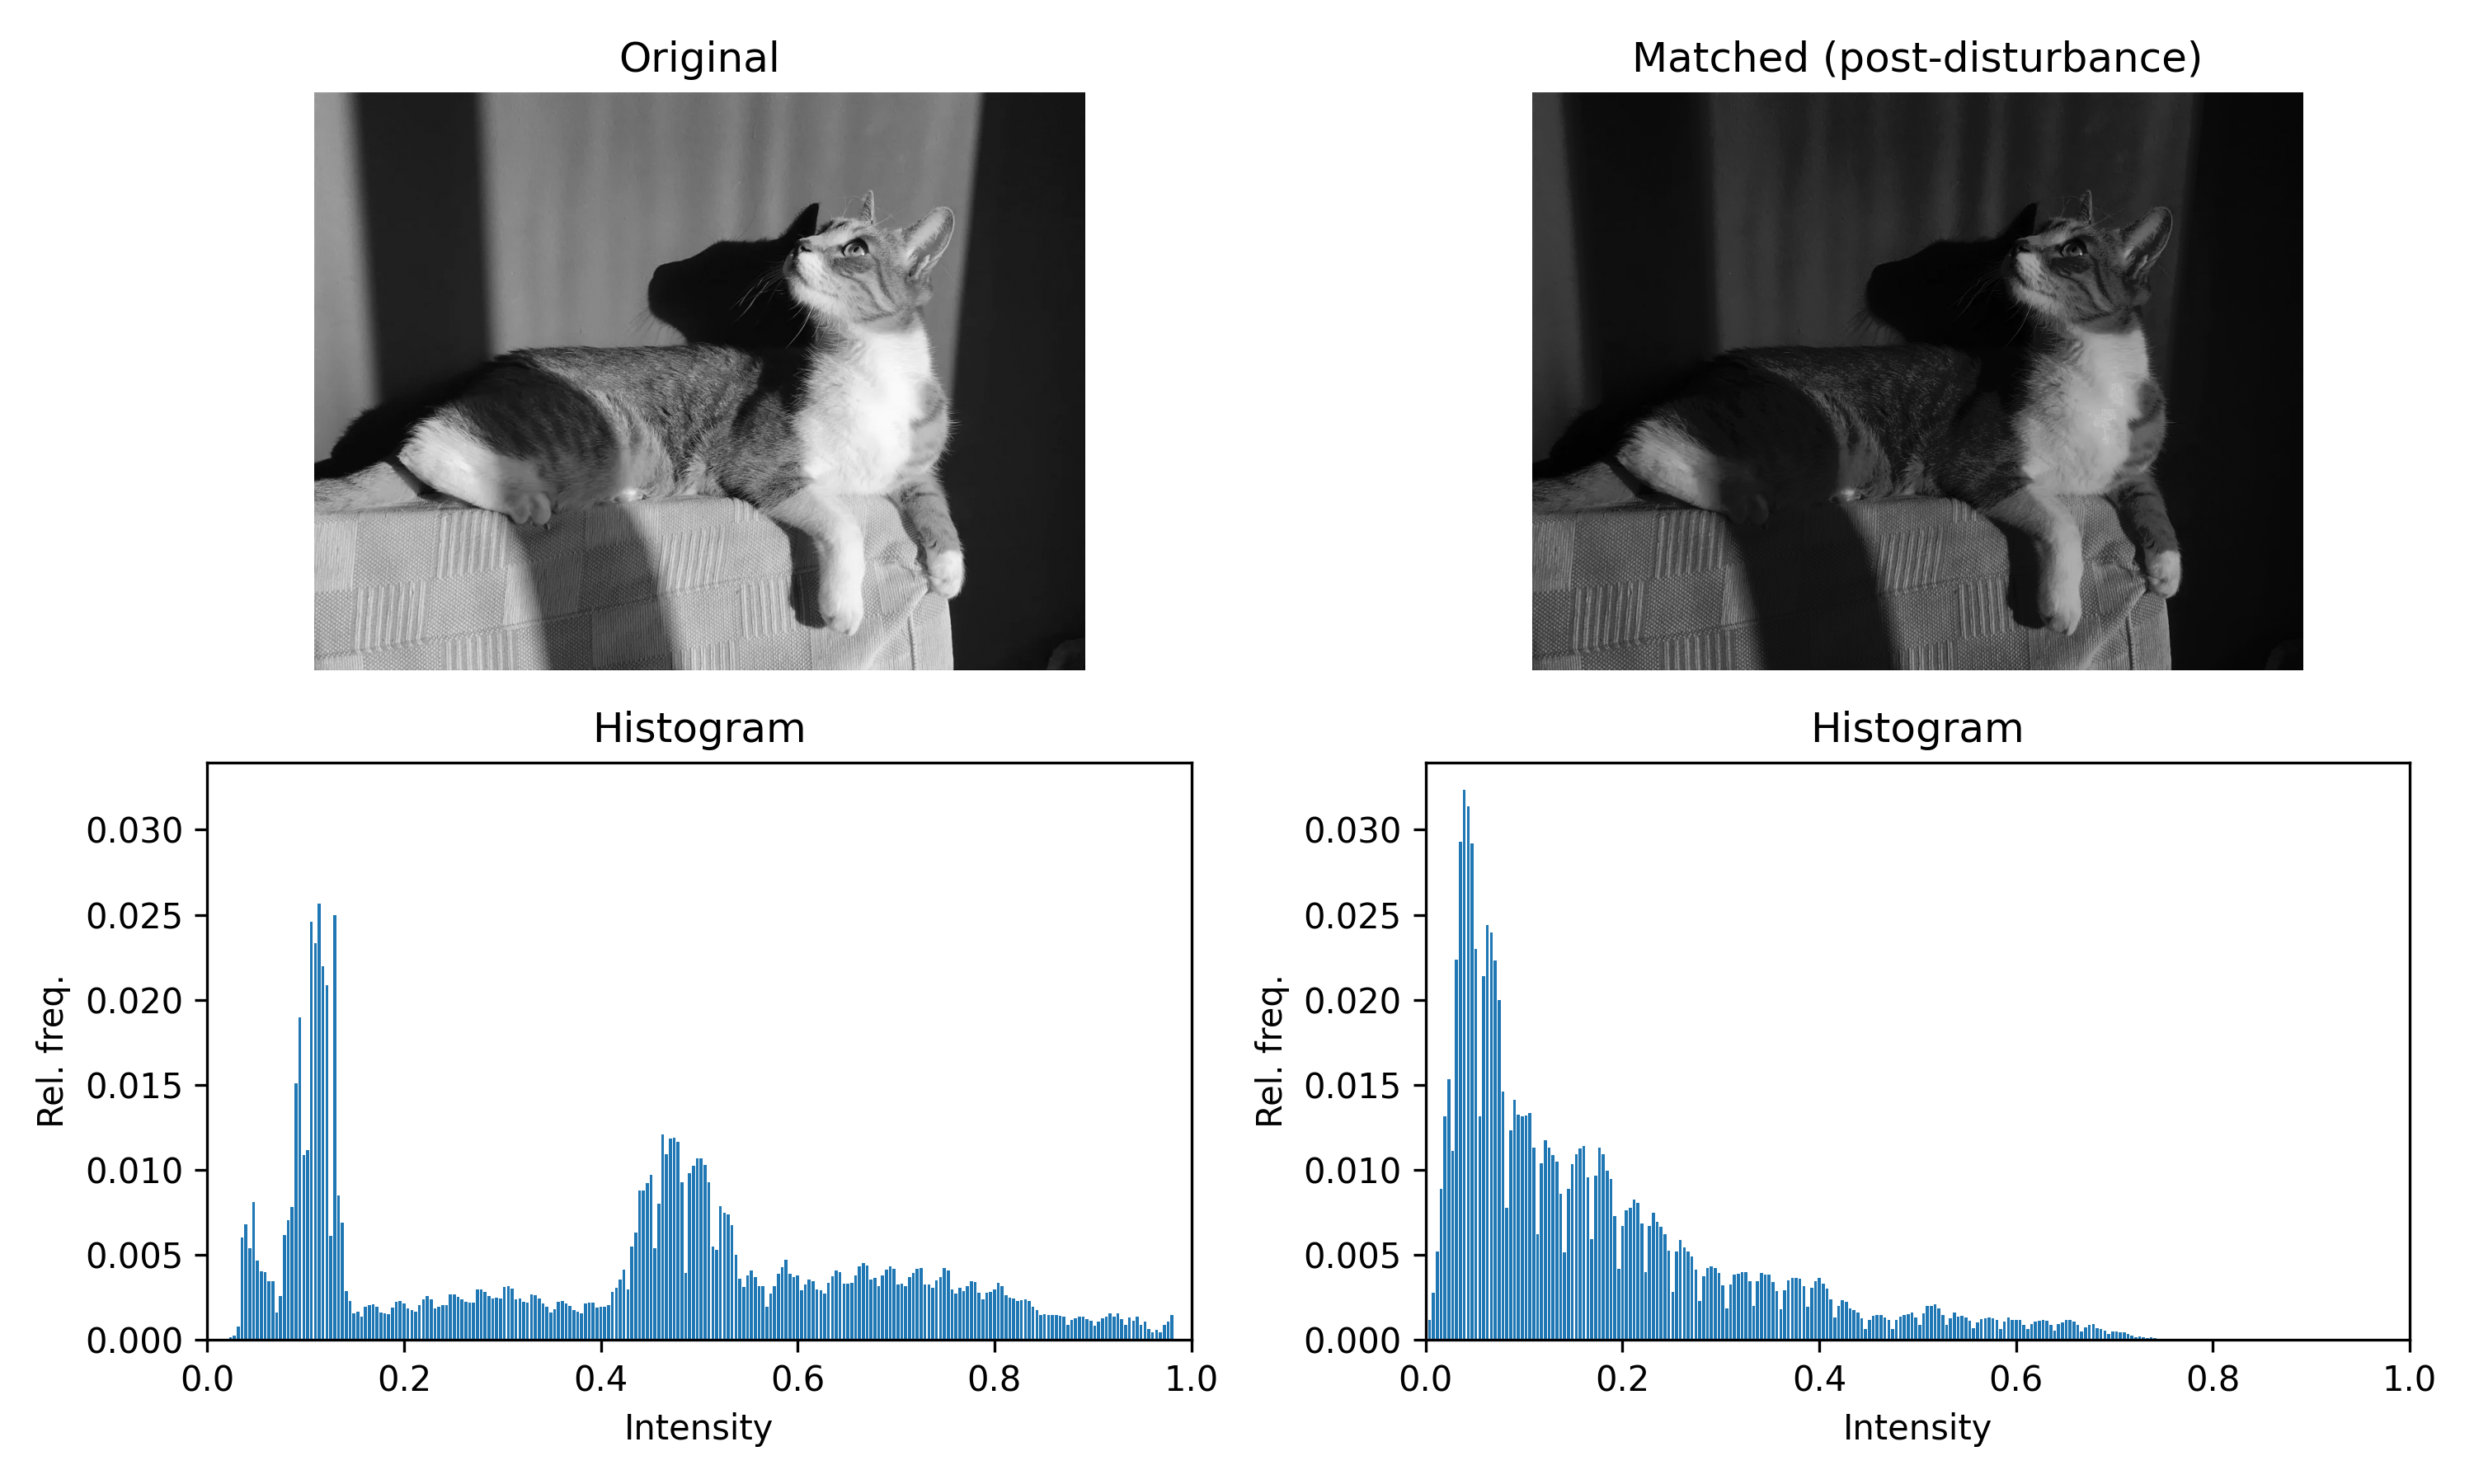
\includegraphics[width=0.9\textwidth]{match_post-disturbance.png}
\caption{Αντιστοίχιση ιστογράμματος με \en post-disturbance\gr. Κατανομή εξόδου παρόμοια με της αναφοράς.}
\end{figure}

\section{Παρατηρήσεις και Συμπεράσματα}

Από τα παραπάνω αποτελέσματα απορρέουν τα εξής συμπεράσματα:
\begin{itemize}
  \item Η μέθοδος \en \textbf{Greedy} \gr τείνει να δημιουργεί απότομα «άλματα» στο ιστόγραμμα λόγω αυστηρής κατανομής με βάση την πληρότητα των \en bins\gr.
  \item Η \en \textbf{Non-Greedy} \gr προσέγγιση εξομαλύνει αυτές τις μεταβάσεις και αποφεύγει υπερβολές.
  \item Η \en \textbf{Post-Disturbance} \gr προσφέρει την πιο ομοιόμορφη κατανομή (ιδανική για εξισορρόπηση), αλλά λόγω θορύβου μπορεί να προκαλέσει ελαφριά απώλεια λεπτομέρειας.
  \item Η διαδικασία αντιστοίχισης \en (matching) \gr καταφέρνει να προσαρμόσει με ακρίβεια την κατανομή της εισόδου με αυτή της αναφοράς, ιδιαίτερα με την προσέγγιση \en post-disturbance\gr.
\end{itemize}

\vspace{0.3cm}

\hspace{-0.6cm}Aξίζει να σημειώσουμε και την επίδραση του πλήθους στάθμεων εξόδου $L_g$ στην εξισορρόπηση ιστογράμματος:

\begin{itemize}
  \item Η παράμετρος $L_g$ ελέγχει το πόσες διαφορετικές στάθμες τιμών θα έχει η έξοδος κατά την εξισορρόπηση.
  \item Για μικρές τιμές $L_g$ (π.χ. 15), η έξοδος εμφανίζει έντονη αφαιρετικότητα, με λίγες διακριτές φωτεινότητες. Αυτό έχει ως αποτέλεσμα εικόνες με αισθητά επίπεδα φωτεινότητας και πολύ «απλοποιημένο» ιστόγραμμα.
  \item Για μεγαλύτερες τιμές $L_g$ (π.χ. 256 ή 1200), η εξισορρόπηση γίνεται πιο λεπτομερής και ομαλή. Η εικόνα εξόδου διατηρεί περισσότερη από την υφή και τα χαρακτηριστικά της αρχικής εικόνας, ενώ το ιστόγραμμα προσεγγίζει καλύτερα την επιθυμητή (συνήθως ομοιόμορφη) κατανομή.
  \item Επομένως, το $L_g$ λειτουργεί ως παράμετρος ρύθμισης της «έντασης» της εξισορρόπησης: μικρό $L_g$ σημαίνει έντονη εξισορρόπηση, μεγάλο $L_g$ σημαίνει πιο λεπτομερή και σταδιακή.
  \item Από τα παραγόμενα ιστογράμματα, παρατηρείται ότι όσο αυξάνεται το $L_g$, τόσο πιο πυκνή και ομοιόμορφη γίνεται η κατανομή των τιμών εξόδου.
\end{itemize}

\hspace{-0.6cm}Συνολικά, το πρόγραμμα καλύπτει όλες τις απαιτήσεις της εκφώνησης, με τεκμηριωμένη υλοποίηση και οπτική επιβεβαίωση των αποτελεσμάτων.

\bibliographystyle{plain}
\begin{thebibliography}{1}
    \bibitem{lnmpikas}
    \en https://numpy.org/doc/
\end{thebibliography}

\end{document}